
\begin{frame}{A generic update engine for dynamic pivoting}
\framesubtitle{Update Issue}
\begin{columns}
\begin{column}{.50\textwidth}
\begin{center}
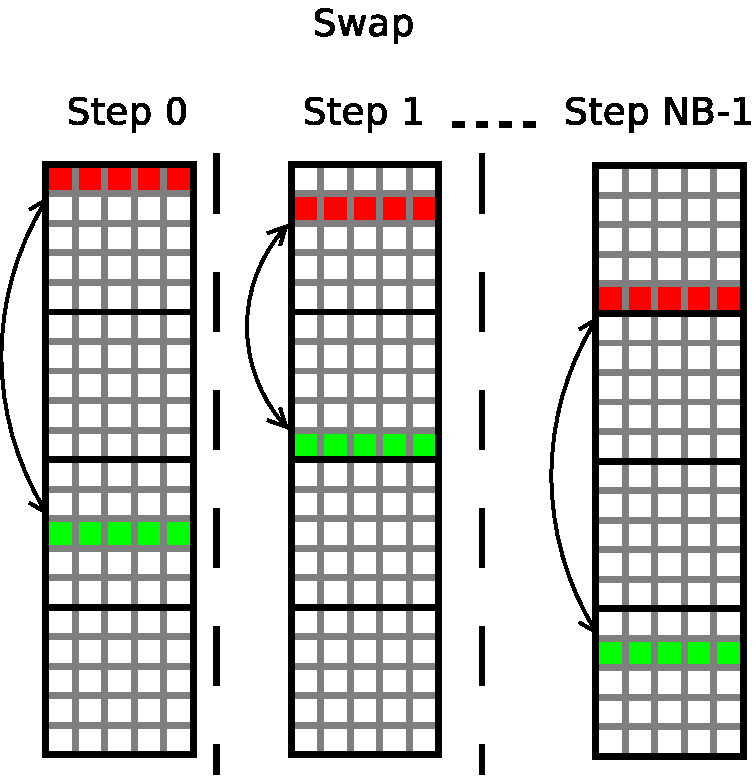
\includegraphics[scale=0.3]{update_swap.pdf}
\end{center}
\end{column}
\hfill
\begin{column}{.50\textwidth}
The tile U exchange swap rows with other concerned tile.
\pause
\begin{exampleblock}{Problem}
\begin{itemize}
\item A dynamic decision for a static DAG \\
$\rightarrow$ Prepare tasks for all possible communications?
\end{itemize}
\end{exampleblock}{}
\end{column}
\end{columns}
\end{frame}

\begin{frame}{A generic update engine for dynamic pivoting}
\framesubtitle{Solutions}
\begin{columns}
\begin{column}{.60\textwidth}
Ideas:
\begin{itemize}
\item Avoiding useless swap to increase parallelism\\
$\rightarrow$ Use of permutations instead of pivots indexes
\transparent{0.4}
\item Updating the main tile is more urgent\\
$\rightarrow$ Parallelize the swap \textbf{from} and the swap \textbf{into} the tile U
\item Minimizing the number of communication (not the volume)\\
$\rightarrow$ Gather communications of all rows over two buffers
\end{itemize}
\end{column}
\begin{column}{.40\textwidth}
\begin{center}
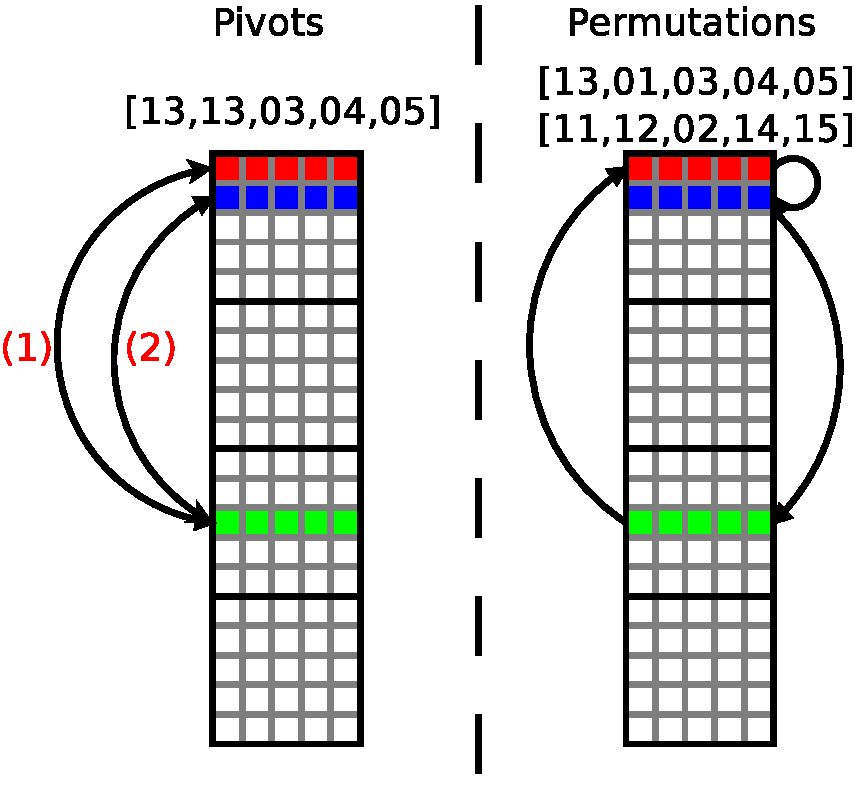
\includegraphics[scale=0.3]{pivots.pdf}
\end{center}
\end{column}
\end{columns}
\end{frame}

\begin{frame}{A generic update engine for dynamic pivoting}
\framesubtitle{Solutions}
\begin{columns}
\begin{column}{.60\textwidth}
Ideas:
\begin{itemize}
{\transparent{0.4}
\item Avoiding useless swap to increase parallelism\\
$\rightarrow$ Use of permutations instead of pivots indexes}
\item Updating the main tile is more urgent\\
$\rightarrow$ Parallelize the swap \textbf{from} and the swap \textbf{into} the tile U
\transparent{0.4}
\item Minimizing the number of communication (not the volume)\\
$\rightarrow$ Gather communications of all rows over two buffers
\end{itemize}
\end{column}
\begin{column}{.40\textwidth}
\begin{center}
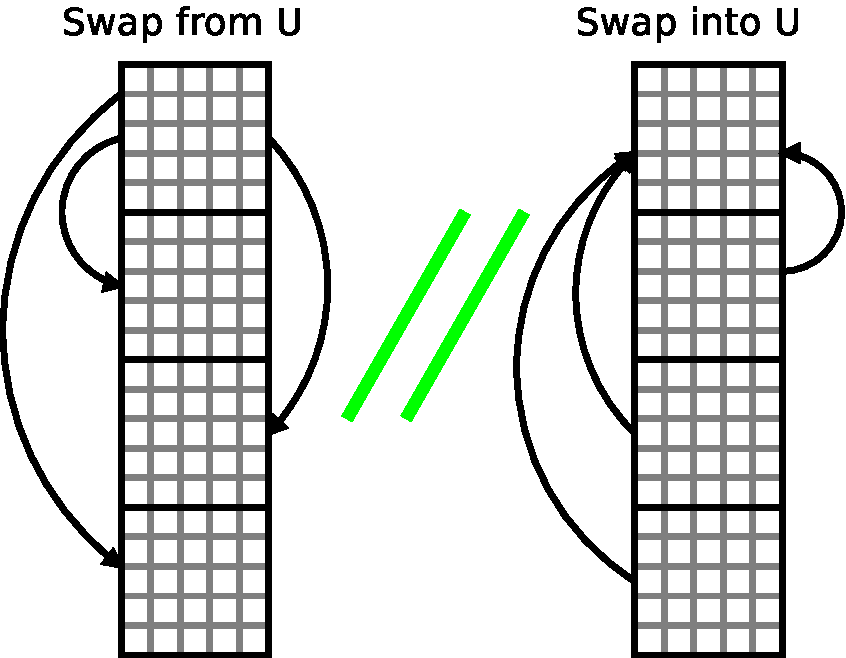
\includegraphics[scale=0.3]{parswap.pdf}
\end{center}
\end{column}
\end{columns}
\end{frame}

\begin{frame}{A generic update engine for dynamic pivoting}
\framesubtitle{Solutions}
Ideas:
\begin{itemize}
\item Avoiding useless swap to increase parallelism\\
$\rightarrow$ Use of permutations instead of pivots indexes
\item Updating the main tile is more urgent\\
$\rightarrow$ Parallelize the swap \textbf{from} and the swap \textbf{into} the tile U
\item Minimizing the number of communication (not the volume)\\
$\rightarrow$ Gather communications of all rows over two buffers
\end{itemize}
\pause
\begin{exampleblock}{}
$\rightarrow$ Five kinds of tasks : COPY, COLLECT, RECEIVE, SEND and PASTE.
\end{exampleblock}{}
\end{frame}

\begin{frame}{A generic update engine for dynamic pivoting}
\framesubtitle{Swap into U}
\begin{columns}
\begin{column}{.60\textwidth}
\begin{itemize}
\item COLLECT: Collecting the lines needed by the tile U into a buffer.
\item SEND: Gather the buffers collected by COLLECT of each node.
\item PASTE: Overwrite the tile U with the buffer.
\transparent{0.4}
\item RECEIVE
\item COPY
\end{itemize}
\end{column}
\hfill
\begin{column}{.40\textwidth}
\begin{center}
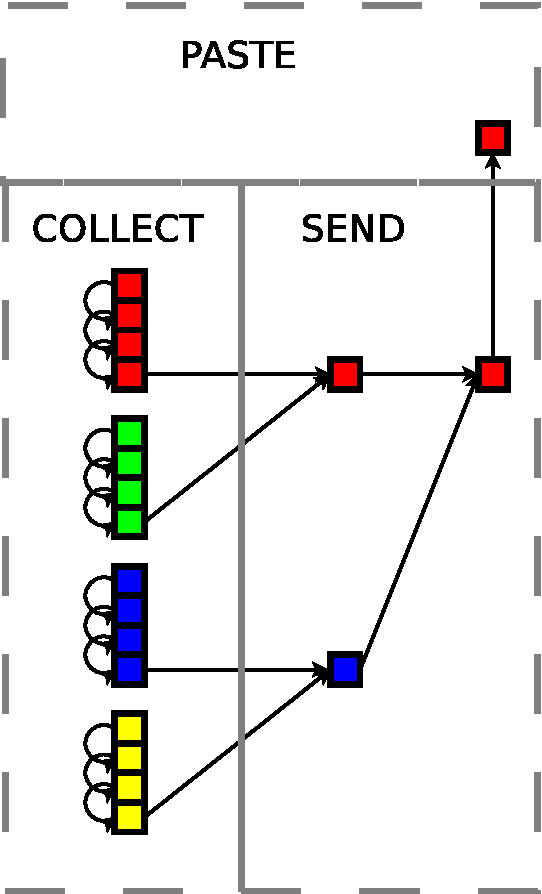
\includegraphics[scale=0.3]{collect.pdf}
\end{center}
\end{column}
\end{columns}
\end{frame}

\begin{frame}{A generic update engine for dynamic pivoting}
\framesubtitle{Swap from U}
\begin{columns}
\begin{column}{.60\textwidth}
\begin{itemize}
{
\transparent{0.4}
\item COLLECT
\item SEND
\item PASTE
}
\item COPY: Copy tile U into a buffer.
\item RECEIVE: Receive the buffer U and make the swap from it.
\end{itemize}
\end{column}
\hfill
\begin{column}{.40\textwidth}
\begin{center}
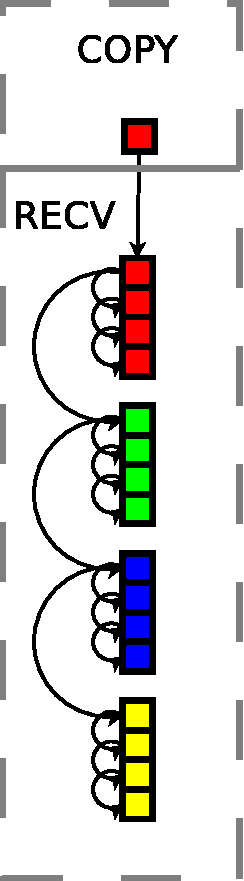
\includegraphics[scale=0.3]{receive.pdf}
\end{center}
\end{column}
\end{columns}
\end{frame}

\begin{frame}{A generic update engine for dynamic pivoting}
\framesubtitle{Update Tasks Synchronisation}
\begin{columns}
\begin{column}{.60\textwidth}
\begin{itemize}
\item COLLECT
\item COPY
\item RECEIVE
\item SEND
\item PASTE
\end{itemize}
\end{column}
\hfill
\begin{column}{.40\textwidth}
\begin{center}
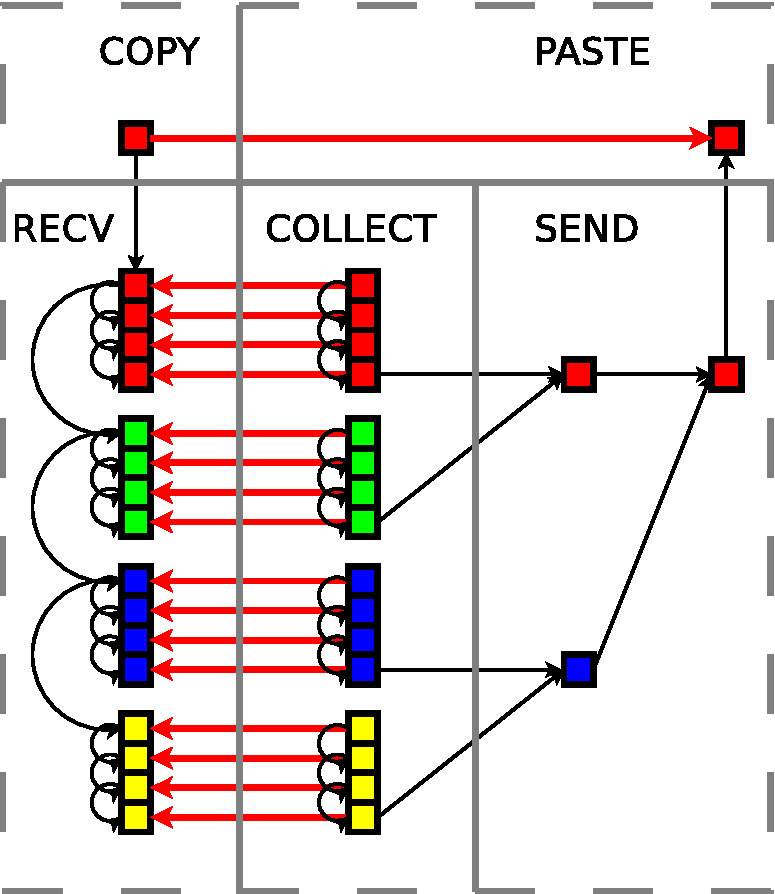
\includegraphics[scale=0.3]{swap_opt.pdf}
\end{center}
\end{column}
\end{columns}
The red arrows prevent the \alert{\textbf{READ AFTER WRITE}}.
\end{frame}

\begin{frame}{A generic update engine for dynamic pivoting}
\framesubtitle{Update Impact}
\begin{center}
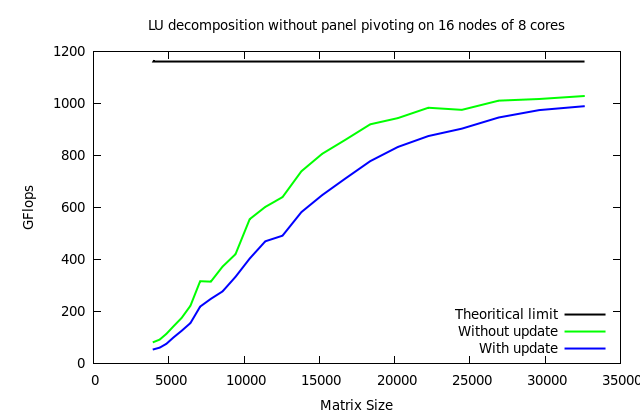
\includegraphics[width=0.7\textwidth]{dgetrf_update_problem.png} 
\end{center}
\end{frame}

\begin{frame}{A generic update engine for dynamic pivoting}
\framesubtitle{Results}
\begin{itemize}
\item Small impact on the performance
\item A generic update engine
\end{itemize}
\end{frame}